\documentclass[a4paper,12pt,openright,notitlepage,oneside]{book}
\raggedbottom % lascia alla fine delle pagine lo spazio invece che adattarle


% pacchetti da caricare
\usepackage[T1]{fontenc} % definisce i caratteri di output
\usepackage{lmodern}
\usepackage[utf8]{inputenc} % definisce i caratteri di input
\usepackage[english]{babel} % definisce la lingua del documento
\usepackage[headheight=15pt]{geometry} % definisce i margini del documento
\geometry{a4paper,top=30mm,bottom=30mm,left=30mm,right=25mm,heightrounded,bindingoffset=3mm}
\usepackage{fancyhdr} % serve per gestire intestazione e piè di pagina
\pagestyle{fancy}
\usepackage{emptypage} % serve per fare le pagine vuote
\usepackage{hyperref} % serve per ottenere links e indice cliccabili
\hypersetup{colorlinks=true,allcolors=black}
\usepackage{microtype} % migliora la scrittura del testo
\usepackage{appendix} % serve per personalizzare l'appendice
\usepackage[printonlyused]{acronym} % serve per creare l'elenco degli acronimi
\usepackage{eurosym} % serve per scrivere il simbolo dell'euro
\usepackage{siunitx} % serve per mettere le unita` di misura nel SI
\usepackage{mathtools} % serve per fare le formule matematiche (carica anche AMSMATH)
\usepackage{booktabs} % serve per fare le tabelle più belle
\usepackage{multirow} % serve per fare le tabelle con righe complesse
\usepackage{pgfplotstable} % serve per fare tabelle da file con dati tabulati
\usepackage{graphicx} % serve per fare le figure
\graphicspath{ {./images/} }
\usepackage{float}
\usepackage{wrapfig} % per poter creare testo attorno alle immagini
\usepackage{tikz} % serve per fare i grafici
\usepackage{pgfplots} % serve a fare i grafici anche lui
\pgfplotsset{compat=1.14}
\usepackage{subcaption} % serve per aggiungere la didascalia alle figure composte (carica anche CAPTION)
\captionsetup{font=small,labelsep=period,format=hang,tableposition=top,figureposition=bottom}
\usepackage{caption}
\usepackage{subcaption}
\usepackage{titlesec}
\usepackage{verbatim}

\titleformat{\chapter}[display]
{\normalfont\bfseries}{}{0pt}{\Large}


% modifiche dei comandi
\renewcommand{\chaptermark}[1]{\markboth{\chaptername\ \thechapter.\ #1}{}} % modifica l'intestazione con il nome/numero del capitolo
\renewcommand{\sectionmark}[1]{\markright{\thesection.\ #1}} % modifica l'intestazione con il nome/numero dela sezione

% nuovi comandi
\newcommand{\R}{\mathbb{R}}
\newcommand{\half}{\frac{1}{2}}
\newcommand{\wrt}{with respect to }
\newcommand{\dof}{deegree of freedom }
\newcommand{\dofs}{deegrees of freedom }
\newcommand{\hot}[1]{\mathcal{O}(#1)}
\newcommand{\ddt}{\frac{d}{dt}}
\newcommand{\equil}[2][x]{\left.\frac{\partial#2 }{\partial #1}\right|_{eq}}
\newcommand{\equilp}[3][x]{\left.\frac{\partial^{#3} #2}{\partial #1 ^{#3}}\right|_{eq}}
\newcommand{\rom}[1]{\uppercase\expandafter{\romannumeral #1\relax}}
\newcommand{\uvec}[1]{\underline{#1}}
\newcommand{\magn}[1]{\left| #1 \right|}
\newcommand{\phase}[1]{e^{i \measuredangle #1}}
\newcommand{\polvec}[1]{\magn{#1} \phase{#1}}
\newcommand{\image} [2] [0.75] {
	\begin{figure}[H]
		\centering
		\includegraphics[width= #1 \textwidth]{#2}
	\end{figure}
	}	


% dichiarazioni personalizzate
\DeclarePairedDelimiter{\abs}{\lvert}{\rvert} % per fare il valore assoluto
\DeclarePairedDelimiter{\norma}{\lVert}{\rVert} % per fare la norma



\begin{document}

	\begin{titlepage}

		% FRONTESPIZIO
		\begin{center}
			% Intestazione
			\Large{\textbf{Politecnico di Milano}} \\
			\vspace{-4mm}
			\rule{\textwidth}{0.4pt}
			\normalsize{AUTOMATION AND CONTROL ENGINEERING} \\
			\vspace{24mm}
			
			% Logo Politecnico
			\begin{figure}[h!]
				\centering
				
\includegraphics[height=0.30\textheight]{images/Template/logo_poli_bianco}
			\end{figure}

			\vspace{25mm}

			% Titolo Tesi
			\huge{\textbf{Study and Control}} \\
			\huge{\textbf{of the Mechanichal System:}} \\
			\huge{\textbf{Rotary Flexible Joint}} \\
			\vspace{15mm}
		\end{center}

		
		\begin{flushright}
			\normalsize{Course} \\
			\small{\textbf{Automation and Control Laboratory}} \\
		\end{flushright}

		\vspace{0.5mm}

		% Autore
		\begin{flushright}
			\normalsize{Student} \\
			\small{\textbf{Andrea Archetti -- 10616682}} \\
			\small{\textbf{Alp Recep Dayan -- 10823110}} \\
			\small{\textbf{Alessandro 	Firetto -- 10633148}} \\
			\small{\textbf{Jesucristo Torres Toledo -- 10822036}} \\
		\end{flushright}

		% Piè Di Pagina
		\begin{center}
			\rule{\textwidth}{0.4pt}
			\small{\textbf{Academic Year 2022 -- 2023}}
		\end{center}
	\end{titlepage}

	\mainmatter % serve per mettere i numeri arabi come numeri di pagina

	% Index
	\tableofcontents

	% Chapters 
	\chapter{Problem Description}
\label{cha:problem_description}

    This report describes our model of the "rotary flexible joint" device made by Quanser and the control schemes we designed to control it.

    The system is composed by a DC motor that provides torque to a metal base, over which a metal arm is fixed with an hinge and two symmetrical springs.

    The length of the arm, hence its inertia, and the equilibrium length of the springs can be modified in a variety of different configurations.

    \image{./images/Chapter 1/system.png}
    The system has several interfaces that could be connected to an acquisition system (ADC/DAC + Amplifier) to acquire measurements and provide input signal, namely:
    \begin{itemize}
        \item Actuators:
            \subitem Voltage driven DC motor;
        \item Sensors:
            \subitem Incremental Encoder for the position of the base \wrt the global reference frame;
            \subitem Incremental Encoder for the relative position of the arm \wrt the base.
    \end{itemize}
    The acquisition system, composed of ADC/DAC + Amplifier model, is out of the scope of this report.

    In the tables below we can see respectively the datasheet for the motor and for the flexible joint:
    \image{./images/Chapter 1/Motor data.png}

    \image{./images/Chapter 1/Flexible joint data.png}

    The main task of this project is to provide a basic control strategy for such system and to develop a more advanced control strategy to accommodate all possible configurations of the system in question.
    
    This goal is divided in sub-tasks to be achieved:
    \begin{enumerate}
        \item Position control of the base, with a frequency based approach;
        \item Position control of the arm tip, with a frequency based and a state space approaches;
        \item Manage uncertainties and control the position of the arm tip with the system in different configurations, with a state space approach and advanced control techniques (robust or adaptive).
    \end{enumerate}






	\chapter{Model Identification}
\label{cha:model_identification}

    The system could be schematized:

    \image{./images/scheme.png}

    It is possible to recognize models of a DC electric motor powered by a voltage $V_{dc}$ coupled with a gearbox (both modeled in the same box) that provide torque $u$ to a flexible (due the springs) joint, at last an encoder to model all the conversion's dynamics between the angular positions $y$ and the red ones $\hat{y}$.

    \section{Mathematical Model Creation}

        \subsection{DC Motor Equations}

            The first task is to decide the shape of the model in terms of which dynamics consider or neglect.

            Starting from the DC motor we assumed a static model due to the fact that from the data sheet of the motor, it should have a dynamic given by the inductance at a frequency:
            \[
                \frac{R}{L} = \frac{2.6 \Omega}{0.18 mH} \approx  15 KHz\]
            this is clearly above the frequency range of the mechanical system, that for its nature should have a frequency in the order at last of $100 Hz$ (deeper treatment in its section).
            
            The physical equations of the Static DC Motor:
            
            \begin{equation*}
                \begin{cases}
                    V_a = R_a I_a + E \\
                    E = k_m \Omega \\
                    \tau = k_t I_a
                \end{cases}
            \end{equation*}

            After several mathematician steps and considering the gearbox effect:

            \[
                \tau = \frac{\eta_m\eta_g k_t K_g(V - K_g k_m\dot\theta)}{R_m} \]
            
            this is the output of the DC Motor's Model, where has been added the gear ratio $K_g$ to provide the angular position at the attaching point of the turret.

        \subsection{Flexible Joint and The Gearbox Equations}

            The model of the beam consider the scheme of the beam as:
            \image{./images/beam_scheme_model.png}
            in this model the system is a 2-dofs mechanical system and can be modeled following a Lagrangian's Approach.

            The 2 \dofs are:
            \begin{itemize}
                \item $\theta$: the absolute angular position of the base of the turret;
                \item $\alpha$: the relative angular position of the tip \wrt to the base of the turret.
            \end{itemize}

            The Kinetic Energy:
            \[
                V = \half J_{eq} \dot{\theta} ^2 + \half J_{L} (\dot{\theta} + \dot{\alpha}) ^2 \]
            where $J_{eq}$ refers to the equivalent inertia of the motor + gearbox, instead $J_{L}$ refers to the inertia of the beam.

            The Potential Energy:
            \[
                V = \half K_s \dot{\alpha}^2\]
            where $K_s$ refers to the linearized stiffness of the equivalent torsional spring. This assumption will be clarified later, but for readability reasons not here.
            
            The Dissipative Function:
            \[
                D = \half B_{eq} \dot{\theta}^2 + \half B_{L} \dot{\alpha}^2\]
            where $B_{eq}$ refers to the equivalent friction of the motor + gearbox, instead $B_L$ refers to the equivalent friction that the single beam is subjected.
            
            Applying the Lagrange treatment for each \dof:
            \begin{equation*}
                \frac{d}{dt} \left(\frac{\partial T}{\partial \dot{x}}\right)-\left(\frac{\partial T}{\partial x}\right)+\left(\frac{\partial D}{\partial \dot{x}}\right)+\left(\frac{\partial V}{\partial x}\right) = \left(\frac{\delta W}{\delta x}\right)\
            \end{equation*}
            and after several mathematical steps the system of equation becomes:
            \begin{equation*}
                \begin{cases*}
                    J_{eq}\ddot\theta+J_{L}(\ddot\theta+\ddot\alpha) + B_{eq}\dot\theta=\tau \\
                    J_{L}(\ddot\theta+\ddot\alpha)+B_L\dot\alpha +K_{stiff}\alpha=0
                \end{cases*}
            \end{equation*}

            \subsubsection{Non-Linear Model for The Spring}

                The reason of considering the couple of spring as an equivalent torsional one is to reduce the complexity of the system.
                The validity of this assumption comes from a study that we did on the error that the linear approximation provides \wrt to the real model.

                Considering the General equation of a spring 
                    \[
                        F = K_s (x_k - x_0)\]
                in the following situations (we consider in this treatment only one spring, but the discussion is valid due to the symmetry for the entire couple)
                \image{./images/non_linear_spring.jpg}
                On the left the equilibrium position $x_k = x_0$, where:
                \[
                    \varphi_0 = atan\left(\frac{P_{1_y}}{P_{0_x}}\right)\]
                \[
                    F_\perp = F \cdot cos(\varphi_0)\]
                \[
                    x_0 = \sqrt{(P_{1_x} - P_{0_x})^2+(P_{1_y} - P_{0_y})^2}\]

                On the right  you are perturbed position, so:
                \[
                    x_k = \sqrt{(P_{1_x} - P_{0_x})^2+(P_{1_y} - P_{0_y})^2} \rightarrow \Delta x_k = x_k - x_0\]
                \[
                    P_1^{NEXT} = \left\lbrack \begin{array}{c}
                        l \cdot cos(\alpha) \\
                        l \cdot (1-sin(\alpha))
                        \end{array}\right\rbrack
                        \rightarrow F_\perp  = F \cdot cos(\varphi + \alpha)\]

                Plotting the value of the $F_\perp$ in function of the angle $\alpha$ compared with a linear increase we obtain:
                \image{./images/K_s_linvs_k_s_NL.png}
                the error between the two curves:
                \image{./images/K_s_linvs_k_s_NL_err.png}

                it is possible to see from the graph that the error starts to be non-negligible above 25 degrees, but from measurements the angle remains under 10 degrees. For this reason we can consider the Force with a linear behavior and the $K_s$ constant.

        \subsection{Development of The State Space Model}
            \subsubsection{Continuous Time}

                Starting from the equations:
                \begin{equation*}
                    \begin{cases}
                        J_{eq}\ddot\theta+J_{L}(\ddot\theta+\ddot\alpha) + B_{eq}\dot\theta=\frac{\eta_m\eta_g k_t K_g(V - K_g k_m\dot\theta)}{R_m} \\
                        J_{L}(\ddot\theta+\ddot\alpha)+B_L\dot\alpha +K_{S}\alpha=0
                    \end{cases}
                \end{equation*}
                we develop the State Space system in continuous time, where the state are:
                \[
                    \left\lbrack \begin{array}{c}
                        \theta \\
                        \dot{\theta} \\
                        \alpha \\
                        \dot{\alpha} 
                        \end{array}\right\rbrack\]
                the matrix A:
                \begin{equation*}
                    \left\lbrack \begin{array}{cccc}
                        0 & 1 & 0 & 0\\
                        0 & -\frac{\eta_m \eta_g k_t k_m K_g^2 +B_{\mathrm{eq}} R_m }{J_{\mathrm{eq}} R_m } & \frac{K_s }{J_{\mathrm{eq}} } & \frac{B_L }{J_{\mathrm{eq}} }\\
                        0 & 0 & 0 & 1\\
                        0 & \frac{\eta_m \eta_g k_t k_m K_g^2 +B_{\mathrm{eq}} R_m }{J_{\mathrm{eq}} R_m } & -K_S \left(\frac{J_{\mathrm{eq}} +J_{L} }{J_{\mathrm{eq}} J_{L} }\right) & -B_L \left(\frac{J_{\mathrm{eq}} +J_{L} }{J_{\mathrm{eq}} J_{L} }\right)
                        \end{array}\right\rbrack 
                \end{equation*}
                and the B matrix:
                \begin{equation*}
                    \left\lbrack \begin{array}{c}
                        0\\
                        \frac{\eta_m \eta_g k_t K_g }{R_m J_{\mathrm{eq}} }\\
                        0\\
                        -\frac{\eta_m \eta_g k_t K_g }{R_m J_{\mathrm{eq}} }
                        \end{array}\right\rbrack
                \end{equation*}

                Considering as the outputs of the system the angular positions $\theta$ and $\alpha$.

            \subsubsection{Discrete Time}
                One last step is to compute the model in discrete time, this is necessary for the last and definitive approach we used in the identification procedure.

                Considering a sampling time $\Delta$ the A matrix:

                \begin{equation*}
                    \left\lbrack \begin{array}{cccc}
                        1 & \Delta  & 0 & 0\\
                        0 & 1-\Delta \frac{\eta_m \eta_g k_t k_m K_g^2 +B_{\mathrm{eq}} R_m }{J_{\mathrm{eq}} R_m } & \Delta \frac{K_{\mathrm{stiff}} }{J_{\mathrm{eq}} } & \Delta \frac{B_L }{J_{\mathrm{eq}} }\\
                        0 & 0 & 1 & \Delta \\
                        0 & \Delta \frac{\eta_m \eta_g k_t k_m K_g^2 +B_{\mathrm{eq}} R_m }{J_{\mathrm{eq}} R_m } & -{\Delta K}_S \left(\frac{J_{\mathrm{eq}} +J_{L} }{J_{\mathrm{eq}} J_{L} }\right) & 1-{\Delta B}_L \left(\frac{J_{\mathrm{eq}} +J_{L} }{J_{\mathrm{eq}} J_{L} }\right)
                    \end{array}\right\rbrack 
                \end{equation*}
                And the B matrix:       
                \begin{equation*}
                    \left\lbrack\begin{array}{c}
                        0\\
                        \Delta \frac{\eta_m \eta_g k_t K_g }{R_m J_{\mathrm{eq}} }\\
                        0\\
                        -\Delta \frac{\eta_m \eta_g k_t K_g }{R_m J_{\mathrm{eq}} }
                    \end{array}\right\rbrack
                \end{equation*}
                the outputs remain the same.

    \section{Identification Technique}

        We proceeded in 3 different way, increasing the complexity, trying to fit as possible all the dynamics of the system. The first two methods didn't provide us enough good results, but are reported because guide us in the choice of a good method for the identification and the model produced is reliable. 
        
        \subsection{Deprecated Methods}
            \subsubsection{Stiffness Identification}
                    
                The first method sticks too much on the reliability of the parameters from the data sheet: we tried to identify just the value of the stiffness of the spring using a step signal and analyzing the frequency of the peak of resonance:
                \[
                    K_s = J_L \cdot \omega_n^2\]
                As result our model didn't fit a lot the real system and the results was so bad that encourage us to proceed in a complete different direction.

            \subsubsection{Identification Toolbox}

                Due to high number of possible uncertainties we look for a different approach that could work around the small number of possible types of experiments and the direct inaccessibility of some parameters. An interesting example of this last consideration is the impossible measurement of the current inside the armature to get a measurement of the resistance $R_m$.

                For these reasons we choose to look for an optimization method that can provide the values of the state space matrices. The first attempt consisted in the usage of the model identification toolbox that, given the order of the system, provides a transfer function representation of the system. 
                
                I will not go in deep with this method became as first step in that direction we didn't put too much effort. In fact, we let Matlab works on its own to get the model however the results weren't good enough and in this way we lost the physical meaning of the provided quantities.

        \subsection{Model Identification using CVX}

            This is the definitive method that we used. CVX is a package allows, giving constraints and objectives, to implement a convex optimization in Matlab in the form:
            \begin{align*}
                \text{minimize   }  & \left\|Ax-b\right\|_{2} \\
                \text{subject to   }& Cx=d \\
                                    & \left\|x\right\|_{\infty} \leq e
            \end{align*}
                
            As dataset we collect the values of the 2 outputs with the system subjected to a square wave of period of $T = 0,63 s$ 
            \image{./images/data_train.png}

            For the optimization we started from the nominal parameters, considering the idea that the real values should be not too far. 
            
            The nominal parameters:

            \begin{itemize}
                \item For the motor:
                    \subitem Motor armature resistance: $R_m = 2.6 \Omega$
                    \subitem Motor current-torque constant: $K_t = 0.00768 Nm/A$
                    \subitem Motor back-emf constant: $K_m = 0.00768 V/(rad/s)$
                    \subitem High-gear total gear ratio: $K_g = 70$
                    \subitem Motor efficiency: $\eta_m = 0.69$
                    \subitem Gearbox efficiency: $\eta_g = 0.9$
                \item The equivalent mechanical system of the motor + gearbox:
                    \subitem Equivalent moment of inertia: $J_{eq} = 0.002087 Kg m^2$
                    \subitem Equivalent viscous damping coefficient: $B_{eq} = 0.015 Nm/(rad/s)$
            \end{itemize}

            For the parameters of the rotating arm we compute the values of the inertia, following its geometry, as:
                \[
                    J_L = m_1 \cdot \frac{L_1^2}{3} + m_2 \cdot \frac{L_2}{12} + m_2 \cdot d^2 = 0.0032 Kg m^2\]
            \image[0.7]{./images/inertia_computation.png}
            the value of the friction coefficient was supposed initially null:
                \[
                    B_L = 0\]
            and the value of the $K_s$ we use the value generated in the analysis stiffness identification:
                
            the analysis provide a Fourier transfer of the second output (the relative position of the tip) as in the figure:
            \image[0.5]{./images/fourier_stiff_analysis.png}
            the peak is at:
            \[
                f = 3.84568 Hz\]
            as result we assign the stiffness initial value as:
            \[
                    K_s = J_L \cdot \omega_n^2 = 1.8426 N/m \]

            
            
            
            
        

                
                




% \section{Research of the machine parameters}
% \label{sec:reserche_machine_parameters}
% The DTC method needs only a few parameters due to the fact that the current saturation is already handled in the computation of the maximum torque and most of the control variables are tuned empirically.
% In fact the 3 needed parameters are:
% \begin{itemize}
%     \item rated speed: 
%             \begin{equation}
%                 \omega_{m_{rated}} = \frac{2\pi f}{n_p} = 104.72 rad/s
%                 \label{eq:omega_m_rated}
%             \end{equation}

%     \item maximum torque:
%             \begin{equation}
%                 me_{max} = \frac{V_{rated}^2}{((\frac{3}{2} (2 \pi f)^2 L_s ((\frac{L_s L_r}{L_m^2})-1)))} = 203.99 Nm
%                 \label{eq:me_max}
%             \end{equation}

%     \item reference stator flux(to use the ferromagnetic material at its maximum):
%             \begin{equation}
%                 \psi_{s_{ref}} = \frac{V_{rated} \sqrt{3}}{2 \pi f} = 2.095 Wb
%                 \label{eq:psi_s_ref}
%             \end{equation}

% \end{itemize}
% \newpage

% \section{Development of the Machine Model}
% \label{sec:machine_model}
% The following scheme in figure \ref*{fig: machine_model} represents the machine model.
% The block scheme uses blocks of Simulink to describe the entire behavior of the motor using differential equations.
% \begin{figure}[h!]
%     \centering
%     \includegraphics[width=1\textwidth]{machine_model.png}
%     \caption{Model of the machine in Simulink}
%     \label{fig: machine_model}
% \end{figure}

% The next ones are all the components used to control the control variables, the 3-phase voltage $V_s$ indeed, and estimate all the control references using the 3-phase vector of the stator current $i_s$.
% Inside the model there are some Complex Integrator that allow to integrete the real part and the imaginary parts of the state vectors separatly and after recompose the originally space vectors.
% \begin{figure}[h!]
%     \centering
%     \includegraphics[width=1\textwidth]{complex_integrator.png}
%     \caption{Scheme of a Complex integrator}
%     \label{fig: complex_integrator}
% \end{figure}
% \newpage

% \section{Development of the Control Unit}
% \label{sec: control_unit}
% The following scheme repreesents the implementation of the controller with the DTC method. This method is based on the dynamic approximation $V_s = \Delta\psi$ that can applies only for high power machine keeping negligible the voltage dissipated on the $R_s$. 
% \begin{figure}[h!]
%     \centering
%     \includegraphics[width=1\textwidth]{DTC_hexagon.png}
%     \caption{Scheme of the stator phase control}
%     \label{fig: DTC_hexagon}
% \end{figure}
% The idea is to keep bounded the magnitude of the $\psi_s$ continuosly switching between different configuation, depending on the sector in which the $\psi_s$ is, (according to $\varphi$) of the 3-phase $V_s$ accorting with the switching table in figure \ref*{fig: switching_table} to keep in rotation the the flux.
% In order to control instead the speed (unless the motor will rotate at the maximum speed) you control the torque, which is controlled by appling null configuaration of the $V_s$ (according to $\tau$) accorting with the switching table in figure \ref*{fig: switching_table}.
% \begin{figure}[h!]
%     \centering
%     \includegraphics[width=0.75\textwidth]{switchin_table.png}
%     \caption{Switching table used in DTC}
%     \label{fig: switching_table}
% \end{figure}
% \\
% The implementation is made by sending to a block that manages the switchin table the two signal $\varphi$ and $\tau$ computed using 2 hysteresis controllers as represented in figure \ref*{fig: hysteresis_controllers}.
% \begin{figure}[h!]
%     \centering
%     \includegraphics[width=0.75\textwidth]{hysteresis_controllers.png}
%     \caption{The hysteresis controllers}
%     \label{fig: hysteresis_controllers}
% \end{figure}
% \\
% In the Simulink implementation is similar to the block scheme, the only differences are:
% \begin{itemize}
%     \item The two side hysteresis for the torque is made with two hysteresis blocks;
%     \item The sector recognition is done evaluating the phase shift of the $\psi_s$;
%     \item The magnitude of the stator flux is evalated comparing the estimated magnitude with a reference value.
% \end{itemize}
% The outputs from these comparisons are the input of a block that implements the switching table as reported in figure \ref*{fig: DTC_controller}.
% \begin{figure}[h!]
%     \centering
%     \includegraphics[width=1\textwidth]{DTC_control_scheme.png}
%     \caption{The DTC control scheme created in Simulink}
%     \label{fig: DTC_controller}
% \end{figure}
% \\
% The inputs of this controller is $m_{e_{err}}$ that is the error of a closed loop control for the torque, where the reference torque is the output of a PI controller that implements a closed loop control for the $\omega_m$, this PI is represented in figure \ref*{fig: speed_controller}. The PI has an anti-windup strategy to avoid saturation's issues with related to the maximum torque.
% \begin{figure}[h!]
%     \centering
%     \includegraphics[width=0.75\textwidth]{speed_controller.png}
%     \caption{The speed controller}
%     \label{fig: speed_controller}
% \end{figure}
% \\
% Another important component is the VI-Estimator that given the the stator current and voltage estimates the stator flux and the torque.
% \begin{figure}[h!]
%     \centering
%     \includegraphics[width=1\textwidth]{VI_estimator.png}
%     \caption{The VI-Estimator}
%     \label{fig: VI_estimator}
% \end{figure}
% The conversion of the Space Vectors into 3-phase components and vice versa are made with the Clark transform and anti-transform.
% \begin{figure}
%     \centering
%     \begin{subfigure}[b]{0.4\textwidth}
%         \centering
%         \includegraphics[width=\textwidth]{clark_transform.png}
%         \caption{Clark transform}
%         \label{fig:clark_transform}
%     \end{subfigure}
%     \qquad
%     \begin{subfigure}[b]{0.4\textwidth}
%         \centering
%         \includegraphics[width=\textwidth]{anti_clark_transform.png}
%         \caption{Clark anti-transform}
%         \label{fig:anti_clark_transform}
%     \end{subfigure}
% \end{figure}



% % \begin{table}[htbp!]
% % \caption{Prima tabella}
% % \label{tab:prima_tabella}
% % \centering
% % \begin{tabular}{cccc}
% % \toprule
% % Prima Variabile	& Seconda Variabile	& Terza Variabile	& Quarta Variabile	\\
% % \midrule
% % XXX				& XXX				& XXX				& XXX				\\
% % \bottomrule	
% % \end{tabular}
% %\end{table}

% % \section{Terza Sezione}
% % \label{sec:terza_sezione_2}
	\chapter{Position Control of the Base}
\label{cha:position_base}

% \section{Research of the machine parameters}
% \label{sec:reserche_machine_parameters}
% The DTC method needs only a few parameters due to the fact that the current saturation is already handled in the computation of the maximum torque and most of the control variables are tuned empirically.
% In fact the 3 needed parameters are:
% \begin{itemize}
%     \item rated speed: 
%             \begin{equation}
%                 \omega_{m_{rated}} = \frac{2\pi f}{n_p} = 104.72 rad/s
%                 \label{eq:omega_m_rated}
%             \end{equation}

%     \item maximum torque:
%             \begin{equation}
%                 me_{max} = \frac{V_{rated}^2}{((\frac{3}{2} (2 \pi f)^2 L_s ((\frac{L_s L_r}{L_m^2})-1)))} = 203.99 Nm
%                 \label{eq:me_max}
%             \end{equation}

%     \item reference stator flux(to use the ferromagnetic material at its maximum):
%             \begin{equation}
%                 \psi_{s_{ref}} = \frac{V_{rated} \sqrt{3}}{2 \pi f} = 2.095 Wb
%                 \label{eq:psi_s_ref}
%             \end{equation}

% \end{itemize}
% \newpage

% \section{Development of the Machine Model}
% \label{sec:machine_model}
% The following scheme in figure \ref*{fig: machine_model} represents the machine model.
% The block scheme uses blocks of Simulink to describe the entire behavior of the motor using differential equations.
% \begin{figure}[h!]
%     \centering
%     \includegraphics[width=1\textwidth]{machine_model.png}
%     \caption{Model of the machine in Simulink}
%     \label{fig: machine_model}
% \end{figure}

% The next ones are all the components used to control the control variables, the 3-phase voltage $V_s$ indeed, and estimate all the control references using the 3-phase vector of the stator current $i_s$.
% Inside the model there are some Complex Integrator that allow to integrete the real part and the imaginary parts of the state vectors separatly and after recompose the originally space vectors.
% \begin{figure}[h!]
%     \centering
%     \includegraphics[width=1\textwidth]{complex_integrator.png}
%     \caption{Scheme of a Complex integrator}
%     \label{fig: complex_integrator}
% \end{figure}
% \newpage

% \section{Development of the Control Unit}
% \label{sec: control_unit}
% The following scheme repreesents the implementation of the controller with the DTC method. This method is based on the dynamic approximation $V_s = \Delta\psi$ that can applies only for high power machine keeping negligible the voltage dissipated on the $R_s$. 
% \begin{figure}[h!]
%     \centering
%     \includegraphics[width=1\textwidth]{DTC_hexagon.png}
%     \caption{Scheme of the stator phase control}
%     \label{fig: DTC_hexagon}
% \end{figure}
% The idea is to keep bounded the magnitude of the $\psi_s$ continuosly switching between different configuation, depending on the sector in which the $\psi_s$ is, (according to $\varphi$) of the 3-phase $V_s$ accorting with the switching table in figure \ref*{fig: switching_table} to keep in rotation the the flux.
% In order to control instead the speed (unless the motor will rotate at the maximum speed) you control the torque, which is controlled by appling null configuaration of the $V_s$ (according to $\tau$) accorting with the switching table in figure \ref*{fig: switching_table}.
% \begin{figure}[h!]
%     \centering
%     \includegraphics[width=0.75\textwidth]{switchin_table.png}
%     \caption{Switching table used in DTC}
%     \label{fig: switching_table}
% \end{figure}
% \\
% The implementation is made by sending to a block that manages the switchin table the two signal $\varphi$ and $\tau$ computed using 2 hysteresis controllers as represented in figure \ref*{fig: hysteresis_controllers}.
% \begin{figure}[h!]
%     \centering
%     \includegraphics[width=0.75\textwidth]{hysteresis_controllers.png}
%     \caption{The hysteresis controllers}
%     \label{fig: hysteresis_controllers}
% \end{figure}
% \\
% In the Simulink implementation is similar to the block scheme, the only differences are:
% \begin{itemize}
%     \item The two side hysteresis for the torque is made with two hysteresis blocks;
%     \item The sector recognition is done evaluating the phase shift of the $\psi_s$;
%     \item The magnitude of the stator flux is evalated comparing the estimated magnitude with a reference value.
% \end{itemize}
% The outputs from these comparisons are the input of a block that implements the switching table as reported in figure \ref*{fig: DTC_controller}.
% \begin{figure}[h!]
%     \centering
%     \includegraphics[width=1\textwidth]{DTC_control_scheme.png}
%     \caption{The DTC control scheme created in Simulink}
%     \label{fig: DTC_controller}
% \end{figure}
% \\
% The inputs of this controller is $m_{e_{err}}$ that is the error of a closed loop control for the torque, where the reference torque is the output of a PI controller that implements a closed loop control for the $\omega_m$, this PI is represented in figure \ref*{fig: speed_controller}. The PI has an anti-windup strategy to avoid saturation's issues with related to the maximum torque.
% \begin{figure}[h!]
%     \centering
%     \includegraphics[width=0.75\textwidth]{speed_controller.png}
%     \caption{The speed controller}
%     \label{fig: speed_controller}
% \end{figure}
% \\
% Another important component is the VI-Estimator that given the the stator current and voltage estimates the stator flux and the torque.
% \begin{figure}[h!]
%     \centering
%     \includegraphics[width=1\textwidth]{VI_estimator.png}
%     \caption{The VI-Estimator}
%     \label{fig: VI_estimator}
% \end{figure}
% The conversion of the Space Vectors into 3-phase components and vice versa are made with the Clark transform and anti-transform.
% \begin{figure}
%     \centering
%     \begin{subfigure}[b]{0.4\textwidth}
%         \centering
%         \includegraphics[width=\textwidth]{clark_transform.png}
%         \caption{Clark transform}
%         \label{fig:clark_transform}
%     \end{subfigure}
%     \qquad
%     \begin{subfigure}[b]{0.4\textwidth}
%         \centering
%         \includegraphics[width=\textwidth]{anti_clark_transform.png}
%         \caption{Clark anti-transform}
%         \label{fig:anti_clark_transform}
%     \end{subfigure}
% \end{figure}



% % \begin{table}[htbp!]
% % \caption{Prima tabella}
% % \label{tab:prima_tabella}
% % \centering
% % \begin{tabular}{cccc}
% % \toprule
% % Prima Variabile	& Seconda Variabile	& Terza Variabile	& Quarta Variabile	\\
% % \midrule
% % XXX				& XXX				& XXX				& XXX				\\
% % \bottomrule	
% % \end{tabular}
% %\end{table}

% % \section{Terza Sezione}
% % \label{sec:terza_sezione_2}
	\chapter{Position Control of The Tip}
\label{cha:position_tip}

% \section{Research of the machine paramethers}
% \label{sec:reserche_machine_paramethers}
% The DTC method needs only a few paramethers due to the fact that the current saturation is already handled in the computation of the maximum torque and most of the control variables are tuned empirically.
% In fact the 3 needed paramethers are:
% \begin{itemize}
%     \item rated speed: 
%             \begin{equation}
%                 \omega_{m_{rated}} = \frac{2\pi f}{n_p} = 104.72 rad/s
%                 \label{eq:omega_m_rated}
%             \end{equation}

%     \item maximum torque:
%             \begin{equation}
%                 me_{max} = \frac{V_{rated}^2}{((\frac{3}{2} (2 \pi f)^2 L_s ((\frac{L_s L_r}{L_m^2})-1)))} = 203.99 Nm
%                 \label{eq:me_max}
%             \end{equation}

%     \item reference stator flux(to use the ferromagnetic material at its maximum):
%             \begin{equation}
%                 \psi_{s_{ref}} = \frac{V_{rated} \sqrt{3}}{2 \pi f} = 2.095 Wb
%                 \label{eq:psi_s_ref}
%             \end{equation}

% \end{itemize}
% \newpage

% \section{Development of the Machine Model}
% \label{sec:machine_model}
% The following scheme in figure \ref*{fig: machine_model} represents the machine model.
% The block scheme uses blocks of Simulink to describe the entire behavior of the motor using differential equations.
% \begin{figure}[h!]
%     \centering
%     \includegraphics[width=1\textwidth]{machine_model.png}
%     \caption{Model of the machine in Simulink}
%     \label{fig: machine_model}
% \end{figure}

% The next ones are all the components used to control the control variables, the 3-phase voltage $V_s$ indeed, and estimate all the control references using the 3-phase vector of the stator current $i_s$.
% Inside the model there are some Complex Integrator that allow to integrete the real part and the imaginary parts of the state vectors separatly and after recompose the originally space vectors.
% \begin{figure}[h!]
%     \centering
%     \includegraphics[width=1\textwidth]{complex_integrator.png}
%     \caption{Scheme of a Complex integrator}
%     \label{fig: complex_integrator}
% \end{figure}
% \newpage

% \section{Development of the Control Unit}
% \label{sec: control_unit}
% The following scheme repreesents the implementation of the controller with the DTC method. This method is based on the dynamic approximation $V_s = \Delta\psi$ that can applies only for high power machine keeping negligible the voltage dissipated on the $R_s$. 
% \begin{figure}[h!]
%     \centering
%     \includegraphics[width=1\textwidth]{DTC_hexagon.png}
%     \caption{Scheme of the stator phase control}
%     \label{fig: DTC_hexagon}
% \end{figure}
% The idea is to keep bounded the magnitude of the $\psi_s$ continuosly switching between different configuation, depending on the sector in which the $\psi_s$ is, (according to $\varphi$) of the 3-phase $V_s$ accorting with the switching table in figure \ref*{fig: switching_table} to keep in rotation the the flux.
% In order to control instead the speed (unless the motor will rotate at the maximum speed) you control the torque, which is controlled by appling null configuaration of the $V_s$ (according to $\tau$) accorting with the switching table in figure \ref*{fig: switching_table}.
% \begin{figure}[h!]
%     \centering
%     \includegraphics[width=0.75\textwidth]{switchin_table.png}
%     \caption{Switching table used in DTC}
%     \label{fig: switching_table}
% \end{figure}
% \\
% The implementation is made by sending to a block that manages the switchin table the two signal $\varphi$ and $\tau$ computed using 2 hysteresis controllers as represented in figure \ref*{fig: hysteresis_controllers}.
% \begin{figure}[h!]
%     \centering
%     \includegraphics[width=0.75\textwidth]{hysteresis_controllers.png}
%     \caption{The hysteresis controllers}
%     \label{fig: hysteresis_controllers}
% \end{figure}
% \\
% In the Simulink implementation is similar to the block scheme, the only differences are:
% \begin{itemize}
%     \item The two side hysteresis for the torque is made with two hysteresis blocks;
%     \item The sector recognition is done evaluating the phase shift of the $\psi_s$;
%     \item The magnitude of the stator flux is evalated comparing the estimated magnitude with a reference value.
% \end{itemize}
% The outputs from these comparisons are the input of a block that implements the switching table as reported in figure \ref*{fig: DTC_controller}.
% \begin{figure}[h!]
%     \centering
%     \includegraphics[width=1\textwidth]{DTC_control_scheme.png}
%     \caption{The DTC control scheme created in Simulink}
%     \label{fig: DTC_controller}
% \end{figure}
% \\
% The inputs of this controller is $m_{e_{err}}$ that is the error of a closed loop control for the torque, where the reference torque is the output of a PI controller that implements a closed loop control for the $\omega_m$, this PI is represented in figure \ref*{fig: speed_controller}. The PI has an anti-windup strategy to avoid saturation's issues with related to the maximum torque.
% \begin{figure}[h!]
%     \centering
%     \includegraphics[width=0.75\textwidth]{speed_controller.png}
%     \caption{The speed controller}
%     \label{fig: speed_controller}
% \end{figure}
% \\
% Another important component is the VI-Estimator that given the the stator current and voltage estimates the stator flux and the torque.
% \begin{figure}[h!]
%     \centering
%     \includegraphics[width=1\textwidth]{VI_estimator.png}
%     \caption{The VI-Estimator}
%     \label{fig: VI_estimator}
% \end{figure}
% The conversion of the Space Vectors into 3-phase components and vice versa are made with the Clark transform and anti-transform.
% \begin{figure}
%     \centering
%     \begin{subfigure}[b]{0.4\textwidth}
%         \centering
%         \includegraphics[width=\textwidth]{clark_transform.png}
%         \caption{Clark transform}
%         \label{fig:clark_transform}
%     \end{subfigure}
%     \qquad
%     \begin{subfigure}[b]{0.4\textwidth}
%         \centering
%         \includegraphics[width=\textwidth]{anti_clark_transform.png}
%         \caption{Clark anti-transform}
%         \label{fig:anti_clark_transform}
%     \end{subfigure}
% \end{figure}



% % \begin{table}[htbp!]
% % \caption{Prima tabella}
% % \label{tab:prima_tabella}
% % \centering
% % \begin{tabular}{cccc}
% % \toprule
% % Prima Variabile	& Seconda Variabile	& Terza Variabile	& Quarta Variabile	\\
% % \midrule
% % XXX				& XXX				& XXX				& XXX				\\
% % \bottomrule	
% % \end{tabular}
% %\end{table}

% % \section{Terza Sezione}
% % \label{sec:terza_sezione_2}
	\chapter{System with uncertainties}
\label{cha:position_tip_uncertanties}

In the last part of our analysis we developed different control schemes to control the position of the tip when the arm had different values of inertia. As we already developed a model for the system in the nominal condition, we can design a control which considers the uncertainties of the parameters in the model and is still able to grant similar performances, and most importantly stability, for all the different system conditions.

In details we are changing the position of the tip of the arm and its value of inertia as expressed in the table below. The inertia is calculated in the same way as in paragraph \ref{sec: param est}.

\begin{table}[h!]
    \centering
    \begin{tabular}{||c c||} 
    \hline
    d[cm] & $J_L[Kgm^2]$ \\ 
    \hline\hline
    20 &  0.0032  \\ 
    \hline
    37 & 0.0062 \\
    \hline
    \end{tabular}
\end{table}

Whereas below we can see the A matrices in continuous time in both cases:

\[
A_{nominal} =
\begin{bmatrix}
    0  &  1.0377    &   -0.6104 &   -7.4061e-5       \\
    0  &  -37.199    &   603.06 &   0.2717       \\
    0  &  -0.0377    &   0.9948 &   1.0001       \\
    0  &  37.201    &   -987.46 &   -0.4496      
\end{bmatrix}   \]
\\
\[
A_{maxInertia} = 
\begin{bmatrix}
    0  &  1.0377    &   -0.6104 &   -7.4053e-5       \\
    0  &  -37.199    &   603.05 &   0.2717       \\
    0  &  -0.0377    &   0.9270 &   1.0001       \\
    0  &  37.201    &   -919.71 &   -0.4183        
\end{bmatrix} 
\]

\section{Robustness of State Space Control}

Knowing that the LQR control has robustness properties, we tried to apply the same control scheme we developed before to the system with different inertia parameters, as it is more reliable than the pole placement controller. 
As the observer relies on a correct model of the system, we decided to slow down the controller to better ensure stability of the closed loop system. 

In the plots below we can see the step response of the system with the maximum possible value of inertia in both cases, $\tau = 10$ and $\tau = 17$.

\begin{figure}[H]
     \centering
     \begin{subfigure}{0.47\textwidth}
         \centering
         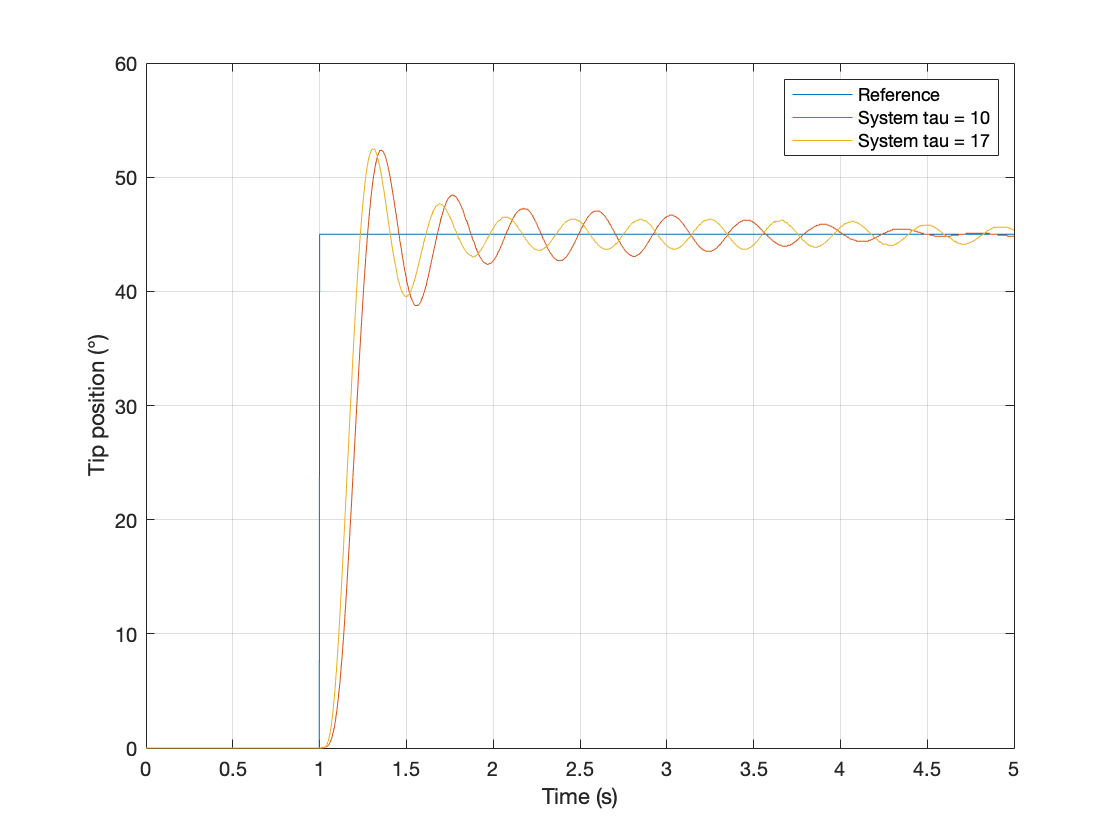
\includegraphics[width=\textwidth]{./images/Chapter 5/LQR/Step_unc.png}
     \end{subfigure}
     \hfill
     \begin{subfigure}{0.47\textwidth}
         \centering
         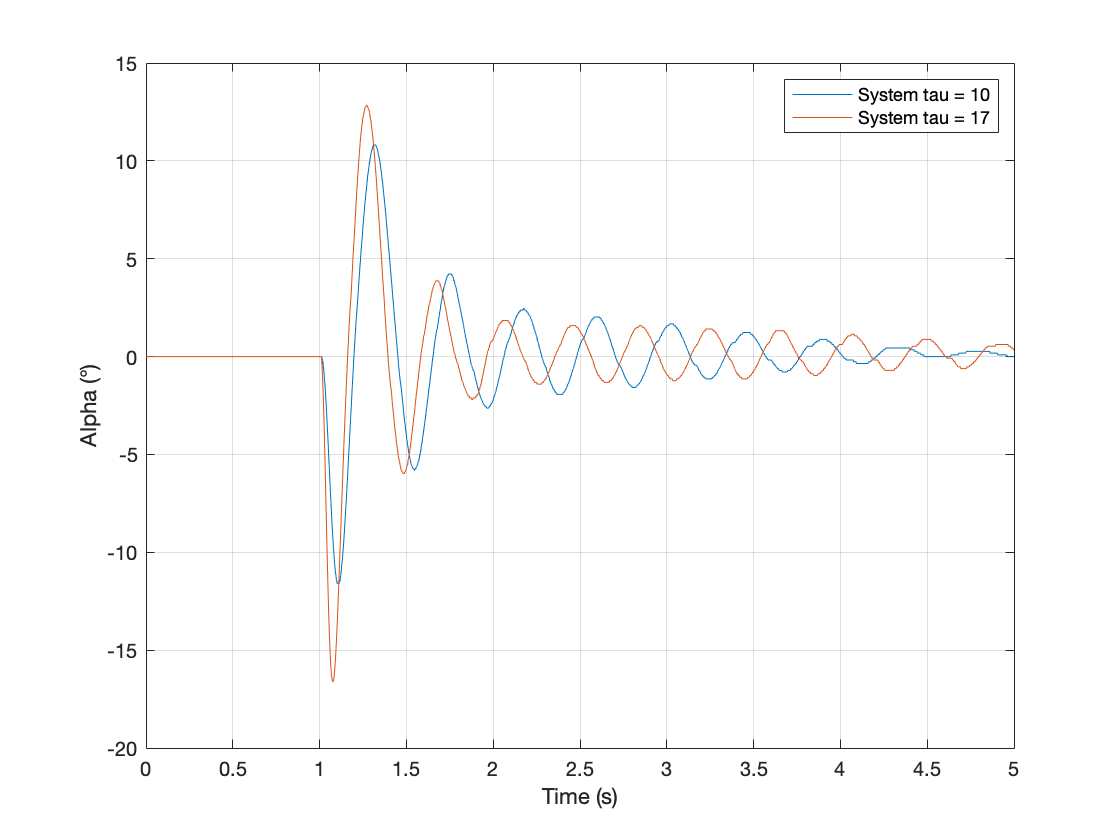
\includegraphics[width=\textwidth]{./images/Chapter 5/LQR/Alpha_unc.png}
     \end{subfigure}
\end{figure}

In the controller design we are not including the uncertainties related to the new system, so we cannot guarantee the same performances as in the nominal case, but still the system is able to reach the reference, although with oscillations.

\section{Robust control}

If we want to consider uncertainties of the model in our design we have to resort to robust control, which means the offline development of a controller that is able to maintain the same performances of the closed loop system even if the model of the system upon which it is designed is not reliable.

\subsection{$H_\infty$ control}

$H_\infty$ control is a type of optimal control scheme which grants robustness if the modeled plant presents uncertainties.

In the image below we can see how the design of the controller is done:

 \image[0.3]{./images/Chapter 5/H_inf/H-infty.png} 

 Where w is the array of exogenous inputs, z is the array of optimization variables, u and v are respectively the inputs and outputs of the enlarged system P and K is the $H_\infty$ controller. 

 In our case w is the reference signal and z is the difference between the reference and the tip position.
 As there was only one value to optimize, the introduction of weights was not necessary in this case.

 The obtained K, which is a 2x1 array of transfer functions, is then implemented as follows:

  \image[1]{./images/Chapter 5/H_inf/Control scheme.png}

Up until now we have a somewhat robust controller for our scheme which works perfectly fine on the nominal system, if we want to also take into consideration the information regarding the uncertainties in the model parameters, then we have to resort to $\mu$ synthesis control.

\subsection{$\mu$ synthesis control}

This kind of control is a generalization of $H_\infty$, the premises and the control scheme are identical but here we can also define a degree of uncertainty for our system, so after applying the controller, the robustness will be the one prescribed.

By looking at the A matrices for the tip position in the maximum inertia case at the beginning of the chapter, we can see that the elements $A(3,3), A(4,3)$ and $A(4,4)$ differ from the nominal case of $\approx 7\%$.

Knowing this information we defined an "uncertain state space" in Matlab having as nominal value the model we found previously and we put an $8\%$ uncertainty on those three parameters inside the A matrix. The $\mu$ synthesis function finds the controller $K_\mu$ by applying the $H_\infty$ algorithm recursively for each value of the parameter inside the specified range and keeping the best one.  

The obtained controller is thus:

\begin{equation*}
    K_\mu= \begin{bmatrix}
        \frac{-362.8 s^3-1.381e4 s^2 - 3.856 e5 s - 5.643 e 6}{s^4 + 81.54 s^3 +3545s^2+7.229e4s+1.329e6}   &
        \frac{-22.8s^3-1019s^2-2.894e4s-4.135e5}{s^4 + 81.54 s^3 +3545s^2+7.229e4s+1.329e6}
    \end{bmatrix}
\end{equation*}

\subsection{Validation}

In the plot below we can see the step response of this new control scheme where the different lines are due to the different values of inertia of the arm. 

 \image[1]{./images/Chapter 5/H_inf/Step.png} 

 As we can see, by increasing the inertia of the system the overshoot increases as well, but still the system is stable and also the performances are roughly the same, regardless of the uncertainties with the nominal model. 

 Unfortunately, when collecting data one of the signal was not starting from 0°, as we can see in the plot, but the conclusions we got are not affected by it, in fact it perfectly behaves like the other signals.

	% Conclusions
	\chapter*{Conclusions}
\label{cha:conclusioni}
\markboth{Conclusions}{}
\addcontentsline{toc}{chapter}{Conclusions}

%Different modeling approaches
\begin{comment}     
        Knowing the state space model of our system we tried 3 different approaches in order to find our system's physical parameters:
        
        \subsection{Deprecated Methods}
            \subsubsection{Stiffness identification}
                    
                The first method sticks too much on the reliability of the parameters from the data sheet: we tried to identify just the value of the stiffness of the spring using a step signal and analyzing the frequency of the peak of resonance:
                \[
                    K_s = J_L \cdot \omega_n^2\]
                As result our model didn't fit a lot the real system and the results was so bad that encourage us to proceed in a complete different direction.

            \subsubsection{Identification Toolbox}

                Due to high number of possible uncertainties we look for a different approach that could work around the small number of possible types of experiments and the direct inaccessibility of some parameters. An interesting example of this last consideration is the impossible measurement of the current inside the armature to get a measurement of the resistance $R_m$.

                For these reasons we choose to look for an optimization method that can provide the values of the state space matrices. The first attempt consisted in the usage of the model identification toolbox that, given the order of the system, provides a transfer function representation of the system. 
                
                I will not go in deep with this method became as first step in that direction we didn't put too much effort. In fact, we let Matlab works on its own to get the model however the results weren't good enough and in this way we lost the physical meaning of the provided quantities.
    \end{comment}

    
\begin{comment}
\section{Adaptive control}

\subsection{Recursive Least Squares}
Recursive least squares (RLS) estimation is a method used in statistical and signal processing to estimate the parameters of a model using a recursive algorithm. It is particularly useful when dealing with time-varying systems where the data arrives sequentially and needs to be processed in real-time.

The RLS algorithm works by iteratively updating the estimated parameters of the model as new data becomes available. It combines the current estimate of the parameters with the new data to obtain an updated estimate that takes into account both past and present information.

%TODO add reference

Considering the A(4,3) and its multiplication with $\dot\alpha$ is roughly 100 times greater than the A(4,4) and $\alpha$. So we decided to estimate the A(4,3) to simplify the estimation process.

state space equation is :
\[ 
x(k+1) = Ax(k) + Bu(k)\\
\]
\[ 
x(k+1,4)= A(4,1)x(k,1) + A(4,2)x(k,2)+A(4,3)x(k,3) + A(4,4)x(k,4) + B(4)u(k)
\]
\[ 
x(k+1,4)-A(4,1)x(k,1)-A(4,2)x(k,2)-A(4,4)x(k,4)-B(4)u(k) = A(4,3)x(k,3)
\]
\[ 
y_{rls}(k+1) = x(k+1,4)-A(4,1)x(k,1)-A(4,2)x(k,2) - A(4,4)x(k,4) - B(4)u(k)
\]
The identification block can be represented as follows. 
\[ 
\hat{\theta}_{rls}(0) = A_{4,3} 
\]
\[ 
u_{rls}(k) = x(k,3)
\]
\[ 
y_{rls}(k) = \hat{\theta}x(k,3)
\]
\[ 
\phi(k) = x(k,3)
\]
\[ 
\hat{\theta}_{rls}(k) =  \hat{\theta}_{rls}(k-1) + V(k)\phi(k)(y_{rls}(k)-\phi(k)'\hat{\theta}(k-1))
\]
\[ 
V(k) = V(k-1) -\frac{V(k-1)\phi(k)\phi(k)'V(k-1)}{1+\phi(k)'V(k-1)\phi(k)}
\]

where $\hat{\theta}_{rls}(k)$ is estimations over time. $u_{rls}(k)$ is input of arx model. $y_{rls}(k) $ is output of arx model. $\phi(k) $ is the regressor. $V(k)$ is the information matrix.
\image{./images/Chapter 5/AdaptivePP/RLSsimulink.png}   

\subsection{Pole Placement with Ackermann}
In simulink the place function is not compiling with quanser. For this reason we implemented Ackermann formula to set the poles for the system every 5 seconds.
\image{./images/Chapter 5/AdaptivePP/AdaptivePP.png}   %TODO: image of pole placement
 We can update the gain to achieve the desired poles in an uncertain change using Ackerman's formula. 
 Firstly, we need to define the characteristic polynomial of the poles. The desired poles are the same as those used previously in  the Pole Placement controller, resulting in the characteristic polynomial:
 \[ 
\Lambda_{desired}(s) = s^4 + 104s^3 + 4046s^2 + 69784s + 450225 
\]
 %insert characteristic polynomial (s)
 Consequently, by substituting the matrix A:
  \[ 
\Lambda_{desired}(A) = A^4 + 104A^3 + 4046A^2 + 69784A + 450225I 
\]
 %insert characteristic polynomial with A
 Then, it is necessary to calculate the controllability matrix using the new matrix A:
 \[ 
M_{c} = [B, AB, A^2B, A^3B]
\]
 %insert controllability matrix
 Finally, from Ackerman's fomula we obtain the  updated $K_{pp}$:
 \[ 
K_{pp} = [0, 0, 0, 1]  M_{c}^{-1}  \Lambda_{desired}(A)
\]
 %Kpp = [0 0 0 1] * inv(R) * {PA}
\subsection{Luenberger Observer}
 The situation in Luenberger observer is different. Here are two outputs used to set the poles. This limits the use of Ackermann. For this reasons we did the pole placement calculations offline on a Matlab script. 
 Since the inertia change depends on the distance of the metal tip, a sweep of different distances are used to calculate the new inertias for the tip. Then using these new inertias new model is created. Then for each model poles are placed and gains are calculated. 
 
 \image{./images/Chapter 5/AdaptivePP/luenberger offline.png}   

Here only changing element in Luenberger gain is L(2,4).
On top of that, L(2,4) and A(4,3) has a R-squared value of 1 stating that these two variables have linear relation. 
In  Simulink block, for estimation of A(4,3) gain is calculated by this linear relation. 

 \image{./images/Chapter 5/AdaptivePP/AdaptiveLO.png}   %TODO: image of observer
Here is the observer block in the Simulink. A martix is updated every 5 second from the output of the RLS block. The gain of observer L(4,2) is retrieved by using updated A(4,2).  

\subsection{Results of Adaptive}
Recursive least squares adaptation requires time to converge so we wanted to see the the convergence on controller. Since settling times are roughly less than 5 seconds controller and Luenberger observer are updated every 5 seconds. Manually we set the covariance matrix in the RLS formulation to 1. This way adaptation is slow enough for us to observed. 

 \image{./images/Chapter 5/AdaptivePP/rlsppsteps.png} 
 
 In this plot overshoots after each update of controller and observer is shown. The starting overshoot was 8.98 percent and then it reduced to 0.78percent at the end. 
 \image{./images/Chapter 5/AdaptivePP/osRLS.png} 
 \end{comment}

\end{document}